\documentclass{article}
\usepackage{color}
\usepackage{graphicx}
\usepackage{setspace}

\usepackage{geometry}
\usepackage{amsmath}
\usepackage{enumitem,amssymb}
\usepackage{pifont}
\geometry{left = 1.25in, right=1.25in} % New Stuff Learned!
\newcommand{\cmark}{\ding{51}}
\newcommand{\xmark}{\ding{55}}
\newcommand{\done}{\rlap{$\square$}{\raisebox{2pt}{\large\hspace{1pt}\cmark}}
\hspace{-2.5pt}}
\newcommand{\wontfix}{\rlap{$\square$}{\large\hspace{1pt}\xmark}}
\newlist{todolist}{itemize}{2}
\setlist[todolist]{label=$\square$}
\doublespacing
\begin{document}
\begin{titlepage}
	

\title{\textbf{ECE358 Week 1}}
\author{\textit{Sanzhe Feng}}
\date{\textit{\today}}
\maketitle
\end{titlepage}
\setlength{\parindent}{0pt}

\textbf{\emph{Asmptotic}} efficiency of algorithms decribes when the size of the input increases without bound.

\section*{3.1 Asymptotic Notation}

\subsection*{Asymptotic notation, functions, and running times}
Asymptotic notation actually applies to functions. For example, the worst-case running time for insertion sort is $an^2+bn+c$, but when we write the asymptotic notation as $\Theta(n^2)$.
\subsection*{$\Theta$-notation}
Definition: For given function $g(n)$, a function $f(n)$ belongs to the \textbf{set} $\Theta(g(n))$ if there exists positive constants $c_1$, $c_2$ and $n_0$ such that $0 \leq c_1g(n)\leq f(n)\leq c_2g(n)$ for all $n \geq n_0$.

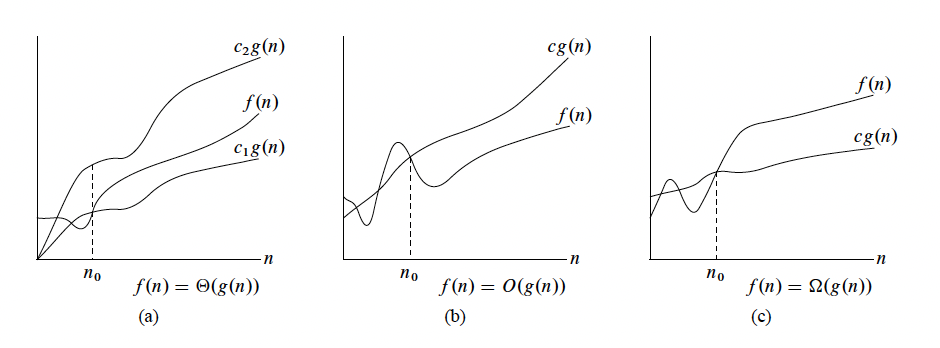
\includegraphics[width=1\linewidth]{P45_3.1.png}
\begin{center}
\small{Figure 1.1 Graphic examples of the $\Theta,$ $\Omega$ and $O$ notations (CLRS P45)}	
\end{center}

Such relationship can be expressed by $f(n) \in \Theta(g(n))$ or $f(n) = \Theta(g(n))$, and $g(n)$ is the \textbf{\textit{asymptotically tight bound}} for $f(n)$. This definition requires that $f(n)$ is nonnegative whenever n is sufficiently large (\emph{\textbf{asymptotically nonnegative}}). Consequently, $g(n)$ needs to be the same way. \\


A formal justification of  $f(n) = \Theta (n)$ where $f(n) = an^2+bn+c$ where $a,b,c$ are constants and $a > 0$. We can easily pick $c_1 = a/4, c_2 = 7a/4$ and $n_0 = 2 \cdot max(|b|/a, \sqrt{|c|/a})$ and verify that 
$0 \leq c_1n^2\leq an^2+bn+c\leq c_2n^2$ (definition). The important thing is that \textbf{some choice exists}. In general, for any polynomial $p(n)=\sum_{i=0}^{k}a_in^i$, we have $p(n) =\Theta(n^d)$ when $a_i$ are constants and $a_d>0$. We can also express constant functions as $\Theta(n^0)$ or $\Theta(1)$.

\subsection*{O-notation}

\textbf{Asymptotic upper bound}. 
Definition: For given function $g(n)$, a function $f(n)$ belongs to the \textbf{set} $O(g(n))$ if there exists positive constants $c$ and $n_0$ such that $0 \leq f(n)\leq cg(n)$ for all $n \geq n_0$. Note that $f(n) = \Theta(g(n))$ \textbf{implies} $f(n) = O(g(n))$ and $f(n) = \Omega(g(n))$. Therefore, if $\Theta (n^2)$, then $O(n^2)$.\\

Suprisingly,we found any linear function $an+b, a>0$ is in $O(n^2)$. This is because in this book, we do not claim about \textbf{HOW TIGHT AN UPPER BOUND IS}. \\

$O$-notation describes an upper bound, when we use it to bound the worstcase
running time of an algorithm, we have a bound on the running time of the algorithm
on \textbf{every input}. Thus, the $O(n^2)$
bound on \textbf{worst-case running time of insertion sort also applies to its running time
on every input}. The $\Theta(n^2)$ bound on the worst-case running time of insertion sort,
however, does not imply $\Theta(n^2)$ bound on the running time of insertion sort on
every input. Since there is an input that makes insertion sort runs in $\Theta(n)$ time. (The simple $\Theta(n^2) \neq \Theta(n^2)$ idea).\\

When we say the running time of insertion sort is $O(n^2)$, we MEAN no matter what the input is, the time is bounded from above by $f(n)$.


\subsection*{$\Omega$-notation}
\textbf{Asymptotic lower bound}. 
Definition: For given function $g(n)$, a function $f(n)$ belongs to the \textbf{set} $\Omega(g(n))$ if there exists positive constants $c$ and $n_0$ such that $0 \leq cg(n) \leq f(n)$ for all $n \geq n_0$.\\

 Based on these three definitions, we can have the following theorem:\\
 {\color{blue}\small \textbf{For any two functions $f(n)$ and $g(n)$, we have $f(n) = \Theta(g(n))$ if and only if $f(n)= O(g(n))$ and $f(n) = \Omega(g(n))$}}\\
 
 The \textbf{running time} of an algorithm is $\Omega(g(n))$ means the running time on any input is \textbf{at least} $g(n)$. In CONCLUSION, the running time of insertion sort belongs to both $\Omega(n)$ and $O(n^2)$ and these bounds are as close as possible: cannot be $\Omega(n^2)$ since \textbf{there is} an input to make the running time $\Theta(n)$ (so $\Omega(n)$).\\
 
 However, we can also say that the worst-case running time of insertion sort is $\Omega(n^2)$ since there does exists an input to make this happen.
 
 
\subsection*{Asymptotic notation in equations and inequalities}
How do we interpret these notations when in equations?

Case 1: When the notation stands alone, the equal sign $=$ means \textit{is a set of }. 

Case 2: When the notation is in a formula, we interpret it as standing for some anonymous function that we do not care to name. e.g. $2n^2+3n+1 = 2n^2+f(n)$ where $f(n)$ is in the set $\Theta(n)$ so we write as $2n^2+3n+1 = 2n^2+\Theta(n)$\\

The number of the anonymous functions (represented by the notations) is understood to be equal to the number of times the notations appears. For example, $\sum_{i=1}^{n}O_i$ can be interpretted as only one single anonymous function (a function of i). {\color{red} What does it even mean though.}\\

Case 3: if the notation is on the left, we interpret it by the following rule:
\textit{No matter how the anonymous
functions are chosen on the left of the equal sign, there is a way to choose
the anonymous functions on the right of the equal sign to make the equation valid. } In the case: $2n^2 +\Theta(n) = \Theta(n^2)$, we interpret it as for any $f(n)\in \Theta(n), $ there is SOME $g(n) \in \Theta(n^2)$ such that $2n^2 +f(n) = g(n)$ for all $n$.
\subsection*{o-notation}


\subsection*{$\omega$-notation}


\subsection*{Relational properties}


\subsubsection*{Transitivity}


\subsubsection*{Reflexivity}


\subsubsection*{Symmetry}


\subsubsection*{Transpose symmetry}


\subsubsection*{Trichotomy}


\section*{3.2 Logarithms}


\section*{Appendix A: Summation}


\end{document}